\chapter{Analýza}
V tejto kapitole sa pozrieme na zopár problémov a ich riešení, na ktoré sme narazili počas vytvárania nášho analyzátoru.
Ako prvé sme sa museli rozhodnúť v akom jazyku budeme náš projekt implementovať. Na to si autor zvolil obecne rozšírený jazyk C++, pretože ho pozná najlepšie a má s ním najviac skúseností. Táto voľba nás zároveň v ničom zásadne neobmedzila a nemala negatívny dopad na celkový výsledok aplikácie. Teraz sa pozrieme na niekoľko konkrétnych problémov a spôsoby akými sme ich vyriešili.

\section{Získanie USB packetov}
Na získavanie USB paketov nám bude obecne slúžiť paket sniffer. Väčšina paket analyzátorov má implementované vlastné sniffery a preto sme sa o to pokúsili tiež. Narazili sme ale na niekoľko zásadných problémov, ktoré sa úzko viažu s platformou na ktorú cielime s našou aplikáciou~--~Windows.

Microsoft dokumentácia podrobnejšie opisuje komunikáciu medzi HID zaridením a kernel/user-mode aplikáciou~\cite{hid_opening_collections}. Pri tejto komunikácii sme schopní zachytiť USB pakety posielané zariadením a neskôr ich analyzovať. Keďže naša aplikácia beží v user-mode, prejdeme si práve tento spôsob komunikácie:
\begin{enumerate}
\item Aplikácia nájde a identifikuje HID zariadenie.
\item Aplikácia pomocou metódy \textit{CreateFile} otvorí spojenie s HID zariadením.
\item Aplikácia pomocou \textit{HID API}~\cite{hid_api} metód \textit{HidD\_Xxx} získa \textit{Preparsed Data} a informácie ohľadom HID zariadenia.
\item \label{kap03:read:paket} \textbf{Aplikácia použije metódu \textit{ReadFile} resp. \textit{WriteFile} na získanie inputu zariadenia resp. poslanie reportu zariadeniu.}
\item Aplikácia pomocou \textit{HID API}~\cite{hid_api} metód \textit{HidP\_Xxx} interpretuje HID reporty.
\end{enumerate}

Podstatný je práve bod~\ref{kap03:read:paket} v ktorom vidíme, že pomocou metódy \textit{ReadFile} sme schopní od daného zariadenia získať USB pakety, ktoré reprezentujú jeho input. Tie by sme následne mohli pomocou nášho analyzátoru spracovať. Tu narážame na prvý problém, ktorý sa priamo viaže na platformu Windows a ktorý si detailnejšie opíšeme v nasledujúcej sekcii.

\subsection{Windows exclusive mód}
Windows má definovaný tzv. \textit{Access Mode}, ktorý určuje restrikciu prístupu \textit{HID Clienta} k HID zariadeniu. 
Ten môže byť buď \textit{Shared} alebo \textit{Exclusive}. \textit{Exclusive Mode} zabraňuje ostatným \textit{HID Clientom} v zachytávaní alebo získavaní inputu HID zariadenia, pokiaľ nie sú hlavným príjemcom daného inputu. Preto z bezpečnostných dôvodov otvára \textit{RIM (Raw Input Manager)} niektoré zariadenia v \textit{Exclusive Mode}.

Ak je zariadenie otvorené v \textit{Exclusive Mode}, aplikácia má stále prístup k niektorým jeho údajom pomocou  \textit{HID API}~\cite{hid_api} metód  \textit{HidD\_\textbf{Get}Xxx}. Tieto metódy nám obecne umožnia získať niektoré descriptory zariadenia, tak ako aj jeho \textit{Preparsed Data}. Nie je nám ale umožnené volať metódu \textit{ReadFile}, takže nemáme akým spôsobom zachytávať komunikáciu HID zariadenia s clientom.

Tabuľka zariadení~\cite{hid_access} (obrázok~\ref{obr:kap3:access_mode}), ktoré \textit{RIM} otvára v \textit{Exclusive Mode} obsahuje aj tie, ktoré sme si v úvode zvolili ako podmnožinu HID zariadení na analýzu -- myš a klávesnica.

\begin{figure}[!htb]
	\centering
	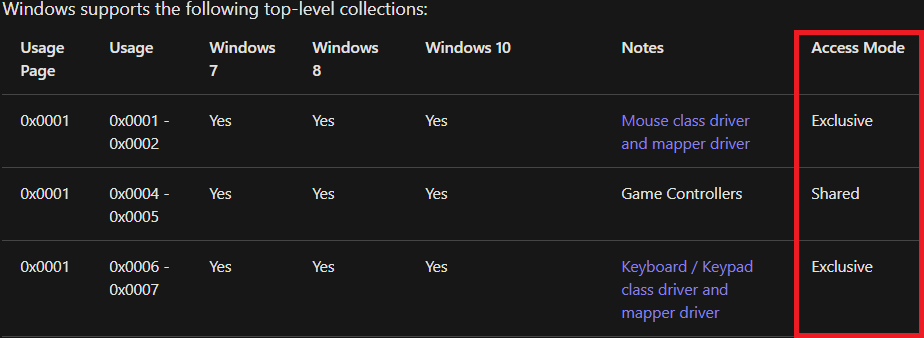
\includegraphics[width=\textwidth]{img/kap3_access_mode}
	\caption{Tabuľka zariadenía ich \textit{Access Mode}. Zariadenia postupne po riadkoch -- myš, joystick a klávesnica}
	\label{obr:kap3:access_mode}
\end{figure}

\subsection{Známe knižnice}
Keďže komunikáciu nemôžeme zachytávať priamo pomocou \textit{HID API}~\cite{hid_api} metód, rozhodli sme sa skúsiť použiť niektoré známe knižnice na sledovanie USB zbernice. 

Pravdepodobne najznámejšou z nich je \textit{libusb}~\cite{libusb} -- knižnica napísaná v jazyku C, ktorá slúži na poskytnutie prístupu k USB zariadeniu. Je cielená na programátorov aby im uľahčila vývoj aplikácií, ktoré komunikujú s USB hardwarom. Podporuje viaceré platformy, medzi ktorými sa nachádza aj Windows. Zároveň beží v user-mode, takže aplikácia ktorá ju využíva nepotrebuje žiadne špeciálne privilégiá na používanie libusb API. Ďalšou výhodou je, že podporuje všetky verzie USB od 1.0 až po 3.1. Je schopná zachytiť všetky typy prenosov (control,bulk,interrrupt,isochronus), a teda by sme pomocou nej mohli sledovať celú komunikáciu so zariadením vrátane počiatočného nakonfigurovania. Bohužiaľ, ani pomocou tejto knižnice sme neboli schopní získať prístup k zariadeniam, ktoré Windows otvára v exclusive móde.

Keďže sa zameriavame na HID zariadenia, skúsili sme hľadať niečo viac špecifické práve pre túto triedu USB zariadení, a to nás zaviedlo k \textit{HIDAPI}~\cite{hidapi_library}. \textit{HIDAPI} je ďalšia veľmi rozšírená knižnica, ktorá umožňuje komunikáciu s USB zariadeniami z HID triedy a takisto beží na viacerých patformách vrátane Windowsu. Pretrváva tu ale rovnaký problém ako s minulou knižnicou -- nie je možné získať prístup k zariadeniam, ktoré sú otvorené vo Windows exclusive móde.

Vyzerá to tak, že jediné riešenie nášho problému je priamo pracovať s filter driverom, ktorý sa nachádza na driver stacku daného zariadenia.

\subsection{Driver}
Windows ponúka niekoľko vstavaných driverov pre rôzne typy zariadení. Stačí ak nájdeme ten, ktorý nám umožní komunikáciu s konkrétnymi HID zariadeniami, s ktorými bol problém kvôli exclusive módu -- klávesnica a myš. Pre tieto dve konkrétne zariadenia momentálne existuje \textit{Moufiltr}~\cite{moufiltr} (upper-level filter driver pre myš) a \textit{Kbfiltr}~\cite{kbfiltr} (upper-level filter driver pre klávesnicu). Tie ale podporujú len legacy zariadenia -- non-USB, non-Bluetooth a non-I2C zariadenia.

Riešením by teda bolo naprogramovanie vlastného filter driveru pre myš a klávesnicu. Toto je ale už nad rámec našej práce a preto na získavanie USB paketov použijeme inú third-party aplikáciu.

\subsection{Third-party aplikácie}
Na zachytávanie USB paketov sme sa rozhodli použiť \textit{USBPcap}~\cite{usbpcap}, s ktorým sme sa už stretli v kapitole~\ref{uvod:sec:Wireshark} keď sme opisovali Wireshark a rôzne sniffery, s ktorými je schopný spolupracovať. USBPcap je veľmi rozšírený Windows sniffer USB paketov a jeho hlavnou výhodou je jednoduchá inštalácia. Takisto nám vyhovuje, že je s ním schopný spolupracovať Wireshark, čo nám častokrát počas vývoja poskytlo spôsob akým sme si mohli overiť správnosť nami vykonanej analýzy niektorých paketov. Daný sniffer zachytáva pakety do súborov v obecne známom formáte -- pcap~\cite{pcap}. 

Miernou nevýhodou je, že nepodporuje čítanie zo súboru do ktorého práve zapisuje -- analýzu paketov v reálnom čase tak budeme musieť vykonať trochu iným spôsobom, a to za pomoci Wiresharku. Ako sme už spomínali, Wireshark je schopný spolupráce s USBPcapom a zároveň podporuje ukladať výstup analýzy do súboru, ktorý je takisto formátu pcap. Wireshark už ale podporuje čítanie z daného súboru počas toho, ako do neho zapisuje. To znamená, že ak budeme chcieť vykonať analýzu v reálnom čase, urobíme to pomocou Wiresharku (konkrétnejší postup si ukážeme neskôr v užívateľskej dokumentácii v kapitole~\ref{udok:chap}).



\section{Sémantická analýza dát}
Ako sme už naznačili v kapitole~\ref{uvod:sec:HID}, na vykonanie sémantickej analýzy inputu HID zariadenia je potrebné získať informácie o danom inpute z Report Descriptoru konkrétneho zariadenia. V tejto kapitole si vysvetlíme formát Report Descriptoru a ako nám informácie ktoré reprezentuje pomôžu v sémantickej analýze inputu HID zariadenia.

\subsection{Report Descriptor}
Celková štruktúra Report Descriptoru je opísaná v HID Class Specification~\cite{report_desc}. Descriptor sa skladá z tzv. itemov, ktoré obsahujú informácie o danom zariadení. Každý item obsahuje hlavičku, ktorá sa skladá z troch častí:
\begin{itemize}
\item Typ
\item Tag
\item Veľkosť
\end{itemize}

Existujú 3 typy itemov : \textit{Main}, \textit{Global} a \textit{Local}. Main item udáva informácie o konkrétnej časti zariadenia (napríklad o tlačidlách na klávesnici, alebo o hodnotách osy X a Y pri pohybe myšou, atď.) Global a Local itemy bližšie špecifikujú Main item (napríklad počet bytov, ktorý je potrebný na reprezentovanie jednotlivých súradníc pri pohybe myšou). Local item určuje vlastnosti len najbližšieho Main itemu, zatiaľ čo Global item je platný pre všetky nasledujúce Main itemy.

Main item má momentálne definovaných 5 tagov:
\begin{itemize}
\item Input -- udáva informácie o inpute zariadenia. Toto je veľmi podstatná časť, pretože práve na základe tohto itemu vieme, že v inpute zariadenia máme očakávať byty reprezentujúce konkrétnu časť zariadenia (bližšie informácie o konkrétnej časti inputu, ako napríklad veľkosť a význam, sú poskytnuté Global a Local itemami pred týmto konkrétnym Input itemom)
\item Output -- podobný význam ako Input item, ale reprezentuje dáta, ktoré sú posielané zariadeniu (napríklad nastavenie LED svetiel na klávesnici)
\item Feature -- itemy ktoré môžu byť posielané ako input aj output a využívajú sa napríklad na kalibráciu konkrétneho zariadenia.
\item Collection -- udáva akúsi logickú kolekciu/zoskupenie rôznych Input/Output/Feature itemov. Napríklad kolekcia myši by mohla obsahovať Input itemy reprezentujúce tlačidlá a súradnice pohybu myši.
\item End Collection -- udáva koniec kolekcie Collection itemu.
\end{itemize}

Vysvetlíme si ešte zopár hlavných Local/Global tagov, ktoré budeme potrebovať aby sme pochopili Report Descriptor:
\begin{itemize}
\item Usage -- reprezentuje odporúčaný význam dát (napríklad, že sa jedná o tlačidlo, osy X/Y/Z, atď.), ale každý výrobca si ho môže definovať po svojom.
\item Usage Page -- zoskupenie jednotlivých Usage-ov do rôznych tried (napríklad Generic Desktop Page, Keyboard Page, LED Page, atď.). Kompletný výpis je dostupný v HID Usage Tables špecifikácii~\cite{usage_pages}. To znamená, že Usage s hodnotou 0x00 môže mať iný význam v Generic Desktop Page ako v Keyboard Page.
\item Report Size a Report Count -- reprezentujú veľkosť dát. Napríklad ak je Report Size = 8 a Report Count = 1, dáta budú reprezentované jednou 8-bitovou hodnotou, takže 1 byte.
\item Logical Minimum a Logical Maximum -- označujú rozsah hodnôt aké môžu dáta nadobúdať.
\end{itemize}

Momentálne keď už máme celkový prehľad o základných itemoch, môžeme si ukázať parsovanie Report Descriptoru na konkrétnom príklade. Na obrázku~\ref{obr:kap3:full_report_desc} môžeme vidieť konkrétny Report Descriptor prevzatý z HID Class Specification~\cite{report_desc_mouse}, reprezentujúci myš. Ten si teraz postupne rozoberieme.

\begin{figure}[!htb]
	\centering
	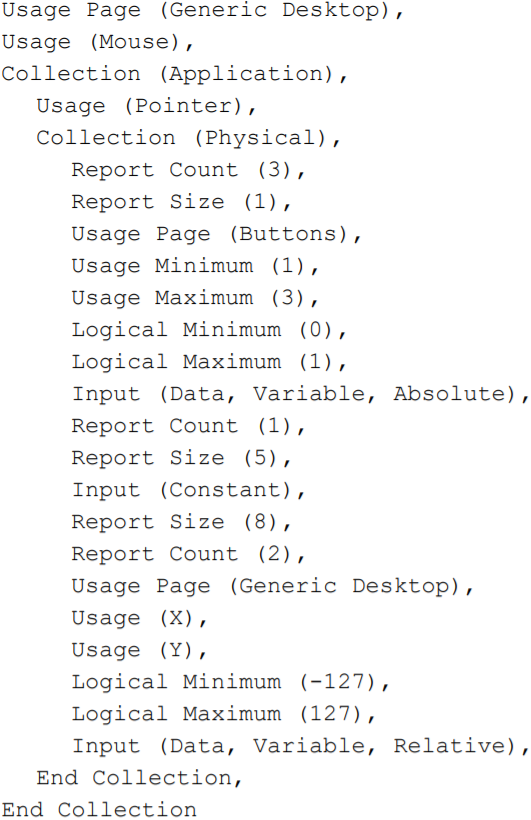
\includegraphics[width=10cm]{img/kap03_full_report_desc}
	\caption{Konkrétny príklad Report Descriptoru myši prevzatý z HID Class Specification~\cite{report_desc_mouse}}
	\label{obr:kap3:full_report_desc}
\end{figure}

\newpage

Z prvej časti (obrázok~\ref{obr:kap3:report_desc_collection}) si môžeme všimnúť, že sa celý Report Descriptor delí do logických kolekcíí -- najprv \textit{Application} a potom \textit{Physical}. Dôležitá je takisto Usage informácia, kde je hneď na začiatku ohraničená Usage Page na \textit{Generic Desktop} a samotný \textit{Usage (Mouse)} nám bližšie špecifikuje, že sa jedná o myš.

\begin{figure}[!htb]
	\centering
	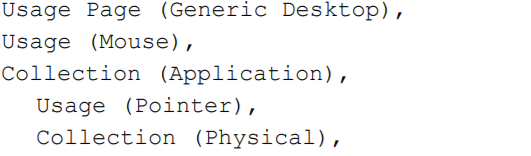
\includegraphics[width=10cm]{img/kap03_report_desc_collection}
	\caption{Časť Report Descriptoru reprezentujúca jednotlivé kolekcie}
	\label{obr:kap3:report_desc_collection}
\end{figure}

Na obrázku~\ref{obr:kap3:report_desc_buttons} vidíme ďalšiu časť descriptoru, ktorá reprezentuje tlačidlá myši -- to sme vyčítali z časti \textit{Usage (Buttons)}. Nasledujúce časti \textit{Report Count (3)} a \textit{Report Size (1)} nám naznačujú, že veľkosť istej podmnožiny dát budú tri 1-bitové hodnoty. Ďalej z hodnôt \textit{Logical Minimum (0)} a \textit{Logical Maximum (1)} vidíme že budú nabývať hodnoty medzi 0 a 1. Nasleduje Input item s hodnotami \textit{Data}, \textit{Variable} a \textit{Absolute} -- tie nám udávajú, že sa jedná o input zariadenia, ktorý bude modifikovateľný (hodnota \textit{Data}), budú to 3 jednotlivé 1-bitové položky (hodnota \textit{Variable}) a hodnota dát nie je relatívna voči inej hodnote (položka \textit{Absolute}). Ďalej vidíme časti \textit{Report Count (1)}, \textit{Report Size (5)} a \textit{Input (Constant)} -- Takže v inpute bude nasledovať časť o veľkosti 5 bitov, ktorá bude mať konštantnú readonly hodnotu (toto v myši väčšinou reprezentuje padding tlačidiel).

\begin{figure}[!htb]
	\centering
	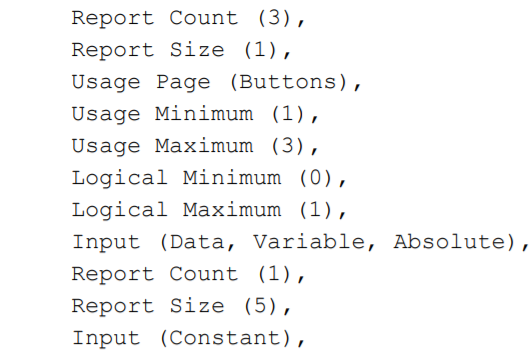
\includegraphics[width=10cm]{img/kap03_report_desc_buttons}
	\caption{Časť Report Descriptoru reprezentujúca tlačidlá myši}
	\label{obr:kap3:report_desc_buttons}
\end{figure}

Z nasledujúcej časti (obrázok~\ref{obr:kap3:report_desc_axis}) vidíme, že sa bude jednať o dve 8-bitové hodnoty (položky \textit{Report Size (8)} a \textit{Report Count (2)}). Následne prepneme Usage Page z \textit{Buttons} na \textit{Generic Desktop} a definujeme 2 Usage pre \textit{X} a \textit{Y} -- tie v myši reprezentujú jednotlivé osy pohybu. Ďalej vidíme, že môžu nadobúdať hodnoty od -127 do 127 (položky \textit{Logical Minimum (-127)} a \textit{Logical Maximum (127)}) čo presne odpovedá rozsahu jedného znamienkového bytu.

\begin{figure}[!htb]
	\centering
	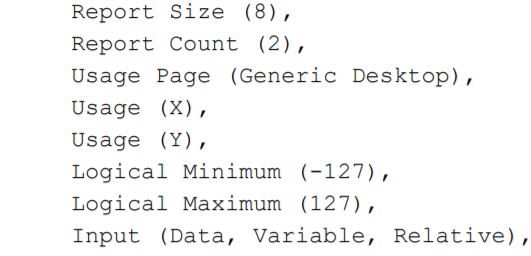
\includegraphics[width=10cm]{img/kap03_report_desc_axis}
	\caption{Časť Report Descriptoru reprezentujúca osy X a Y pri pohybe s myšou}
	\label{obr:kap3:report_desc_axis}
\end{figure}

Na poslednom obrázku~\ref{obr:kap3:report_desc_end} už len vidíme ukončenie kolekcií, tak ako aj celého Report Descriptoru.

\begin{figure}[!htb]
	\centering
	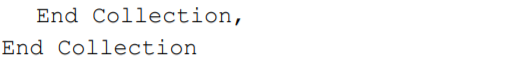
\includegraphics[width=10cm]{img/kap03_report_desc_end}
	\caption{Časť Report Descriptoru reprezentujúca ukončenie jednotlivých kolekcií}
	\label{obr:kap3:report_desc_end}
\end{figure}

V konečnom dôsledku nám z toho teda vychádza, že input našej myši bude mať veľkosť 3 byty (sčítanie všetkých \textit{Report Size} * \textit{Report Count}), kde prvé 3 bity budú reprezentovať stlačenie tlačidiel, nasledujúcich 5 bitov bude výplň a posledné 2 byty reprezentujú osy X a Y v tomto poradí. Toto reprezentuje jeden input report nášho zariadenia na jeho konkrétnom endpointe. Jeden endpoint ale môže obsahovať viac reportov (či už input, output alebo feature). V takom prípade musia byť jednotlivé reporty prefixované 1B hodnotou, ktorú nazývame \textit{Report ID} a ktorá musí byť uvedená v Report Descriptore pri jednotlivých reportoch v podobe \textit{Report ID} itemu. Ako príklad niečoho takého si môžeme predstaviť klávesnicu so zabudovaným zariadením s funkciou myši. Takáto klávesnica môže posielať informácie o stlačení kláves tak ako aj o pohybe myši v jednom endpointe. Na rozlíšenie o ktoré dáta sa jedná by sa použil Report ID.

Ostáva nám ešte jedna možnosť, ktorú sme doteraz nespomenuli -- ako priradiť Report Descriptor k jednotlivým reportom pokiaľ ich zariadenie posiela z viacerých endpointov. To si vysvetlíme v nasledujúcej sekcii.

\subsection{Report Descriptor $\longleftrightarrow$ endpoint}
Ako už vieme z kapitoly (ODKAZ), jedno USB zariadenie môže pozostávať z viacerých interfacov. Každý interface má dané endpointy, ktoré sa s ním viažu. Pri komunikácii medzi USB hostom a zariadením si z hlavičky jednotlivých paketov vieme vytiahnuť informáciu do ktorého endpointu zapisujeme, resp. z ktorého endpointu čítame dáta. Takže v prípade reportu poslaného zariadením vieme zistiť k akému endpointu sa viaže. Hodilo by sa nám teda vedieť k jednotlivým endpointom priradiť im odpovedajúci Report Descriptor. Túto informáciu máme nepriamo poskytnutú v Setup Pakete, ktorý posiela USB host v momente keď si od zariadenia vypýta jeho Report Descriptor. Špecifikuje v ňom totiž položku \textit{wInterfaceNumber}, ktorá udáva číslo interfacu pre ktorý si USB host vypýtal Report Descriptor. Teraz nám už len stačí zistiť aké endpointy sa na daný interface viažu -- túto informáciu sme zíkali vyššie v konfigurácii keď si USB host vypýtal od zariadenia Configuration Descriptor a spolu s ním dostal aj Interface Descriptor a jemu odpovedajúce Endpoint Descriptory.



\section{Voľba frameworku}
obecne co by som od toho GUI priblizne chcel, potom opisat preco som si vybral prave Qt a v nasledujucich kapitolach opisat rozhodnutia uz v Qt
dovod preco som si zvolil qt namiesto inych c++ GUI frameworkov(napriklad sfml)


\section{Spracovávanie pcap súborov}
moznosti ako citat pcap subory : bud pouzit uz existujucu kniznicu : na linuxe Libpcap, windows NPcap(deprecated WinPcap), alebo citat subory manualne : std::istream alebo QFile
\section{Zobrazenie základných informácií}
ako zobrazovat zakladne info o packete : pouzit QListWidget alebo QTableWidget (pripadne nieco ine ako nejaky abstract viewmodel), narok na zakladne funkcionality : lahka rozsiritenlnost o dalsie ''stlpceky'' , moznost jednoduchej interakcie(doubleClick na polozku). Mat vsetky info na jednom okne / mat pop-up okna. Farebne oddelenie.
\section{Zobrazenie sémantického významu dát}
ako vyzobrazit semanticky vyznam roznych dat - descriptory, usb header, vyznam input dat roznych HID zariadeni
\section{Hexdump}
ako v qt urobit hexdump - do coho zobrazovat data(vytvorit si vlastny viewer dedeny od QAbstractScrollArea, pripadne niecoho ineho) vs najst nieco co uz v qt je a upravit to aby to sedelo poziadavkam. Vziat do uvahy bezne funkcie hexdumpu : selection mody(oznacit naraz hexa a im odpovedajuce printable), logicke oddelenie dat(napriklad farbami)








